\documentclass{citask}

% -- PREAMBLE --
\usepackage{float}
\usepackage{graphicx}
% Pakiety do diagramu
\usepackage{tikz}
\usetikzlibrary{shapes,arrows,positioning}

\graphicspath{{images/}} % Set the path for your figure images

\begin{document}

% -- TITLE PAGE --
% Define the title page information before the \makefrontpage command!

\title{Analysis of heart rate variability using mobile devices and machine learning}% Title of the article

\authors{
  \author
  {Jan Kosma Bancerewicz, Julian Jerzy Kotłowski, Ostap Lozovyy, Julia Beata Morawska, Mateusz Rzęsa}% Author name and surname
  {Faculty of Electronics, Telecommunications and Informatics, Gdańsk University of Technology}% Name of the institution
  {Gabriela Narutowicza 11/12, 80-233, Gdańsk, Poland}% Address of the institution
}

\abstract{
  This paper presents methods of heart rate variability analysis based on electrocardiographic and photoplethysmographic signals obtained using mobile devices. An approach to processing the recorded data involving noise suppression, peak detection, and determining inter-pulse intervals in the physiological signal was developed. Detection of R peaks in ECG and maxima of a PPG wave was performed using convolutional and recurrent neural networks. The accuracy of the models was measured in comparison to the classic algorithms and reference data. The results show a high accuracy of peak identification and allow employing mobile devices to monitor cardiac parameters in home environments, particularly under resting-state conditions.
}
% #2 removed "both home environments and during physical activities.", because our app cannot measure above 100bpm
\keywords{heart rate variability; photoplethysmography; convolutional neural networks;}

\makefrontpage{}

% -- DOCUMENT BODY --
% Organize your document as You wish


\section{Introduction}
Heart rate variability (HRV) is an important parameter in assessing cardiovascular health, as it reflects the balance between the sympathetic and parasympathetic nervous systems. Traditional measurements conducted in clinical settings are characterized by high precision and stability, utilizing specialized heart rate monitors to acquire photoplethysmographic or electrocardiographic measurements. However, these clinical methods are often limited by high costs and restricted recording durations.
% issue #2 added info about resting state conditions (below)

In recent years, advances in mobile technology have enabled the monitoring of cardiac activity in daily life. In mobile applications, the signal quality is generally sufficient for use in home environments, while maintaining the advantages of universality, low cost, and broad hardware accessibility. To balance these benefits with the need for high signal fidelity required for accurate HRV estimation, this study focuses on system validation under resting-state conditions.
% issue #1 "Przenieść ogólne opisy pulsometrów i mobile health z opisu aplikacji (Sekcja 3.1.2) do Wstępu (Introduction)"


\subsection{Aim of the study}
The aim of this study is to evaluate whether a low-cost, mobile photoplethysmographic acquisition system supported by deep learning–based beat detection can provide heart rate variability measurements comparable to those obtained from an electrocardiographic reference. Specifically, the study investigates the accuracy and robustness of classical peak-detection algorithms and neural network models when applied to both signals, with the goal of determining their suitability for reliable HRV estimation in real-world conditions. To achieve this objective, resting-state PPG recordings captured by an Android smartphone application are validated against synchronous ECG measurements acquired using the Polar H10 sensor, serving as the reference device. The comparison focuses on the precision of peak detection and the consistency of computed cardiac interval metrics.

\paragraph*{Paper structure.}
The remainder of the paper is structured as follows. Section 2 reviews the theoretical background of analytical and modeling methods in biomedical signal processing. Section 3 characterizes the proposed system architecture, including the signal processing pipeline and neural network models. Section 4 details the experimental setup, data acquisition procedures, and dataset organization. Section 5 evaluates the performance of the proposed methods and discusses the experimental results. Finally, Section 6 summarizes the study and outlines limitations as well as directions for future research.

%\newpage
% Techniki filtracji i modelowania sygnałów biomedycznych
\section{Filtration and biomedical signals modeling techniques}
Electrocardiography and photoplethysmography are among the most fundamental sources of biomedical signals used in modern diagnostic and monitoring systems. The signal processing is aimed at ensuring the reliability of physiological data in the presence of interference such as patient movements, environmental noise, and hardware limitations. Two dominant approaches are used: data filtering and artificial intelligence-based modeling. These approaches are often combined to improve the accuracy and robustness of the analysis in clinical settings \cite{1}.

% Filtracja danych
\subsection{Data filtration}
Initial processing of physiological signals is based on interference elimination, improving the signal-to-noise ratio (SNR). Measurement errors caused by motion artifacts, power line interference at 50/60 Hz, and baseline wander are major sources of distortion in electrocardiography and photoplethysmography \cite{2}. Filtering enhances signal quality and improves the accuracy of feature detection as well as classification performance.

% -> KOREKTA Rozwinięcie skrótów 
A band-pass filter restricting the frequency band to values characteristic of the given waveform is a fundamental method in signal analysis. The processing range is 0.5–40 Hz for ECG signals and 0.3–8 Hz for PPG signals, corresponding to the heart rate \cite{3}. Butterworth, Chebyshev, and elliptic filters, implemented in both infinite impulse response (IIR) and finite impulse response (FIR) forms, are used in digital applications. FIR filters modeled using the window method provide stability and a linear phase response \cite{4}.

Adaptive filters are applied to signals containing disturbances with varying parameters. LMS and RLS algorithms enable dynamic adaptation of system coefficients to signal characteristics, increasing the effectiveness of suppressing motion artifacts and power line interference. Notch filters are used to suppress the 50/60 Hz component \cite{5}.

Pulse artifacts and short-term impulse artifacts are suppressed using a median filter as well as morphological methods, which preserve diagnostic features such as QRS complexes \cite{6}. Empirical Mode Decomposition, Wavelet Packet Transform, and wavelet analysis enable signal decomposition into frequency components and selective noise suppression while preserving the structure of measurement peaks \cite{7}.

In advanced biomedical devices, algorithms based on probabilistic models are used. One such method is the Kalman filter, which estimates the actual measurement based on noise-affected observations \cite{8}. Another method is Independent Component Analysis, employed to separate signal sources and eliminate motion artifacts in photoplethysmography \cite{9}. Modern data isolation techniques combine traditional computing with machine learning. Signal refinement precedes feature extraction with neural networks, which increases the robustness of analysis under real-world conditions \cite{10}.
% W zaawansowanych zastosowaniach biomedycznych wykorzystuje się algorytmy oparte na modelach probabilistycznych. Jedną z metod jest filtr Kalmana, służący do estymacji rzeczywistego przebiegu na podstawie obserwacji obarczonych zakłóceniami \cite{8}, oraz Independent Component Analysis, stosowaną do separacji źródeł zapisu i eliminacji zniekształceń ruchowych w fotopletyzmografii \cite{9}. Współczesne techniki wyodrębniania danych integrują tradycyjne przetwarzanie z uczeniem maszynowym. Proces oczyszczania sygnału jest etapem poprzedzającym ekstrakcję cech z użyciem sieci neuronowych, zwiększając odporność analizy w warunkach naturalnych \cite{10}.
\subsection{Machine learning}
Artificial intelligence-based techniques represent one of the key approaches in biomedical signal analysis. The application of such algorithms enables automatic information extraction, reduces the reliance on preprocessing, and improves classification performance in the presence of interference.

\subsubsection{Traditional Machine Learning}
Traditional supervised approaches are widely utilized for heart rate measurement and arrhythmia detection. Algorithms such as Support Vector Machines (SVM), k-Nearest Neighbors (k-NN), and Random Forests classify signal features based on labeled training data. Additionally, logistic regression and linear discriminant analysis (LDA) provide simple and effective identification of signal patterns. The implementation of these methods in mobile diagnostic systems and monitoring devices, as well as their real-time processing, is enabled by their low computational complexity \cite{11}.

Beyond standard classification, probabilistic models are used to handle sequential data. Hidden Markov Models (HMMs) are employed to identify anomalies and improve the effectiveness of dynamic heart rate analysis as well as the detection of cardiological abnormalities \cite{13}.

\subsubsection{Deep Learning Approaches}
Deep learning architectures offer advanced capabilities for capturing complex dependencies in electrocardiographic and photoplethysmographic signals. Sequential models, specifically Recurrent Neural Networks (RNNs) and their extended forms—Long Short-Term Memory (LSTM) networks and Gated Recurrent Units (GRUs)—are designed to capture both short-term and long-term temporal variations in the signal \cite{12}.

Convolutional Neural Networks (CNNs) are commonly used to extract local features, such as peak detection in PPG signals and QRS complexes in ECG signals \cite{14}. More recently, Transformer models based on the attention mechanism provide parallel mapping of temporal dependencies at multiple scales, increasing the system's robustness against motion artifacts and amplitude variability \cite{15}. Hybrid solutions, in which convolutional layers are combined with recurrent layers to integrate both local and global features within a single system, are also gaining increasing relevance.

A key advantage of these deep learning approaches is their ability to adapt to new datasets. The transfer of models trained on large reference datasets to real-world clinical conditions is achieved through transfer learning, improving both generalization and classification accuracy \cite{16}.

% Ocena zmienności rytmu serca na podstawie przebiegów EKG i PPG
\subsection{Heart rate variability assessment based on ECG and PPG waveforms}
Photoplethysmographic signals are commonly used to estimate heart rate, while electrocardiography serves as the reference standard. The literature features both multichannel PPG datasets with parallel ECG recordings and ultra-short-term HRV analyses performed using deep learning algorithms.

End-to-end approach to evaluating heart rate variability parameters from 10-second fragments of optical measurements was developed in the Wang and Najafizadeh study \cite{17}. To recreate the necessary features a recurrent LSTM neural network was employed. Cardiographic reference signal was registered using a standard clinical system. Acquired coefficients of correlation to reference values exceeded 0.9 with average relative error below 10\% which signifies a high accuracy of the model for any minimal-length sample.

The UTSA-PPG dataset \cite{18} was published in 2025. It contains hours-long recordings of photoplethysmographic signals with parallel electrocardiographic measurements, supplemented with accelerometer data. Heart rate analysis showed an average deviation of less than 2 beats per minute, and the correlation with ECG for basic HRV indicators ranged from 0.85 to 0.95, depending on the metric used. Machine learning techniques, including decision trees and multilayer perceptrons, were employed for signal processing, enabling precise profile reconstruction. Integrating these models into a hybrid approach improved accuracy and reduced error. The variety of samples supports the development of architectures capable of high generalization.

De Ridder et al. \cite{19} conducted a systematic review of mobile applications based on optical pulse measurements, which acquire data in contact mode with a sampling frequency determined by the frame rate. Validation studies in controlled environments confirmed strong agreement between heart rate values and cardiac signals, with consistency levels ranging from 0.95 to 0.99 and an absolute error below 2 beats per minute \cite{20}. A lower fit was observed for short deviation intervals, with correlation values of 0.75–0.85. Results deteriorated further in everyday environments due to motion artifacts, necessitating the use of filtering and data correction procedures to handle distorted signals.

\subsection{Reference Algorithms: Pan-Tompkins}
The Pan-Tompkins algorithm is a classic method for R-peak detection in ECG signals, widely used as a baseline for comparison. It is based on multi-step processing: the first phase involves band-pass suppression of low and high-frequency distortionary components. Waveform differentiation enhances the steep slopes of the QRS complex. Subsequently, the mean of the squared samples is computed in a moving integration window. The final peak detection is realized using analysis of the integrated curve and local maximums \cite{27}.

%Opis systemu i danych
%Akwizycja danych
%Akwizycja danych EKG
\section{System and data characterization}
This section outlines the comprehensive system architecture designed for heart rate variability (HRV) analysis. The solution integrates signal acquisition, preprocessing, and advanced machine learning techniques to ensure robust performance. The workflow begins with data acquisition from dual sources: video input for photoplethysmography (PPG) and chest-strap sensors for electrocardiography (ECG). The raw data undergoes signal extraction and digital filtration to remove noise and motion artifacts. Subsequently, the processed signals are segmented and fed into a hybrid deep learning model combining Convolutional Neural Networks (CNN) and Long Short-Term Memory (LSTM) layers. The model output allows for precise peak detection, which serves as the basis for the final Heart Rate Variability (HRV) calculation. The complete data processing pipeline is illustrated in Figure~\ref{fig:system_diagram}.

%\ref{fig:system_diagram}
%TODO dopisac o diagramie, wkleic diagram, dodac opis

\begin{figure}[htbp]
    \centering
    \resizebox{!}{0.45\textheight}{
    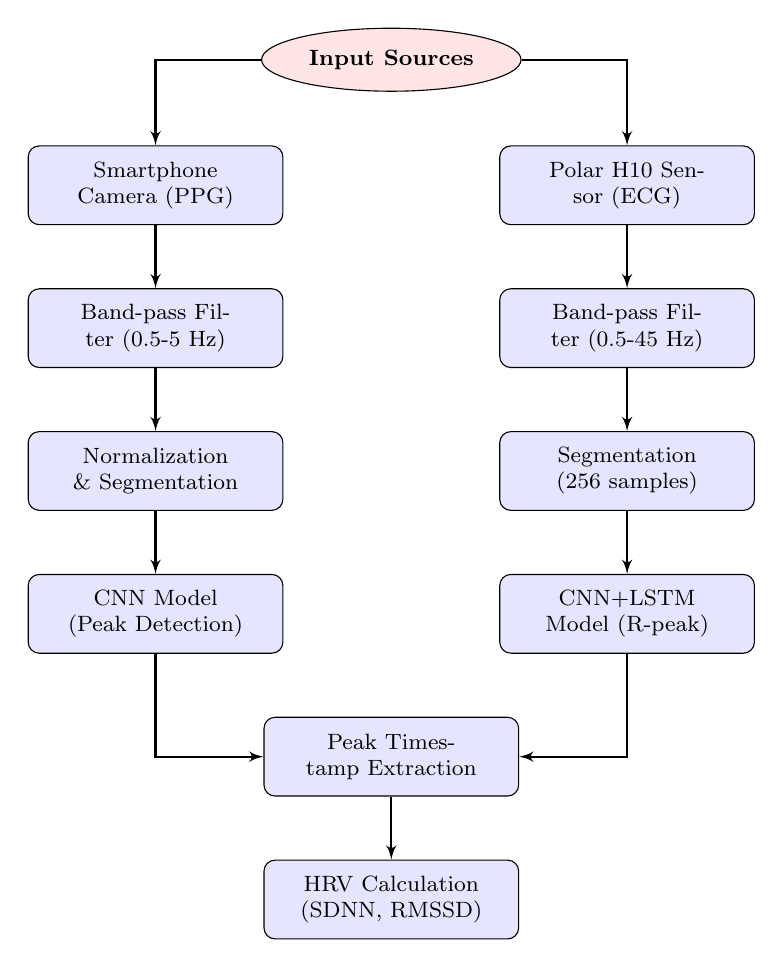
\begin{tikzpicture}[
        node distance=0.8cm and 0.5cm, 
        auto,
        block/.style={
            rectangle, 
            draw, 
            fill=blue!10, 
            text width=3cm, 
            text centered, 
            rounded corners, 
            minimum height=1cm,
            font=\footnotesize
        },
        cloud/.style={
            draw, 
            ellipse, 
            fill=red!10, 
            minimum height=0.8cm,
            font=\footnotesize\bfseries
        },
        line/.style={draw, -latex', thick}
    ]
        % -- Węzły (Nodes) --
        
        % Wejście
        \node [cloud] (input) {Input Sources};
        
        % Lewa kolumna (PPG)
        \node [block, below left=0.8cm and 0.2cm of input] (camera) {Smartphone Camera (PPG)};
        \node [block, below=of camera] (ppg_filt) {Band-pass Filter (0.5-5 Hz)};
        \node [block, below=of ppg_filt] (norm) {Normalization \& Segmentation};
        \node [block, below=of norm] (cnn) {CNN Model (Peak Detection)};
        
        % Prawa kolumna (ECG)
        \node [block, below right=0.8cm and 0.2cm of input] (polar) {Polar H10 Sensor (ECG)};
        \node [block, below=of polar] (ecg_filt) {Band-pass Filter (0.5-45 Hz)};
        \node [block, below=of ecg_filt] (seg) {Segmentation (256 samples)};
        \node [block, below=of seg] (cnn_lstm) {CNN+LSTM Model (R-peak)};
        
        % Połączenie (Merge) - wyliczamy środek pod kolumnami
        \path (cnn.south) -- (cnn_lstm.south) coordinate[midway] (center_point);
        \node [block, below=0.8cm of center_point] (peaks) {Peak Timestamp Extraction};
        
        % Wynik
        \node [block, below=of peaks] (hrv) {HRV Calculation (SDNN, RMSSD)};
        
        % -- Ścieżki (Paths) --
        
        % Od góry do kolumn
        \path [line] (input) -| (camera);
        \path [line] (input) -| (polar);
        
        % Połączenia w kolumnach
        \path [line] (camera) -- (ppg_filt);
        \path [line] (ppg_filt) -- (norm);
        \path [line] (norm) -- (cnn);
        
        \path [line] (polar) -- (ecg_filt);
        \path [line] (ecg_filt) -- (seg);
        \path [line] (seg) -- (cnn_lstm);
        
        % Połączenia do wspólnego bloku (zakrzywione)
        \path [line] (cnn.south) |- (peaks.west);
        \path [line] (cnn_lstm.south) |- (peaks.east);
        
        % Koniec
        \path [line] (peaks) -- (hrv);
        
    \end{tikzpicture}
    }
    \caption{Block diagram of the proposed HRV analysis pipeline. The system processes ECG and PPG signals in parallel streams, applying specific filtering and deep learning models to extract peak timings for final HRV metric calculation.}
    \label{fig:system_diagram}
\end{figure}


\subsection{Data acquisition}
\subsubsection{ECG data acquisition}
Data used for R-peak detection model training and validation was acquired using the Polar H10 heart monitor, which is capable of recording electrocardiographic signals at a sampling frequency of 130 Hz. This resolution enables the creation of a profile essential for HRV analysis.
% Dane wykorzystane do trenowania i walidacji modelu detekcji załamków R zostały pozyskane za pomocą pulsometru Polar H10, zdolnego do rejestrowania sygnału elektrokardiograficznego z częstotliwością próbkowania wynoszącą 130 Hz. Przyjęta wartość umożliwia charakterystykę przebiegu istotną dla analizy HRV.

The Polar H10 sensor is a heart rate detector commonly used in sports and diagnostics. The device employs chest electrodes to register electric potentials associated with cardiac activity, providing higher measurement precision compared to optical methods. Data transmission is carried out via the Bluetooth Low Energy (BLE) standard, while internal memory allows offline storage of recordings. The accuracy of the Polar H10 is comparable to that of single-channel ECG systems used in clinical diagnostics, making mobile signal acquisition feasible \cite{21}.
%Sensor Polar H10 jest czujnikiem tętna stosowanym w sporcie oraz diagnostyce. Działanie urządzenia opiera się na elektrodach piersiowych rejestrujących potencjały elektryczne związane z aktywnością serca, zapewniając wyższą precyzję pomiaru w porównaniu z metodami optycznymi. Transmisja przebiegu realizowana jest poprzez standard Bluetooth Low Energy, a pamięć wewnętrzna umożliwia zapis danych w trybie offline. Dokładność detekcji Polar H10 jest zbliżona do systemów EKG jednokanałowych stosowanych w diagnostyce klinicznej, umożliwiając zastosowanie w mobilnym rejestrowaniu sygnału \cite{21}.

% 7# korekta odnośnie data acquisition
To collect the training dataset, eight measurement sessions were conducted with five participants. Each recording contained approximately 230,000 samples, corresponding to about 30 minutes of continuous signal per session. Data was transmitted in real time in 13-point packets, consistent with the established sampling rate, and subsequently stored in CSV format. These recordings captured varied heart rate dynamics and were used exclusively for model training to prevent data leakage.
%W celu zebrania zbioru treningowego przeprowadzono osiem sesji pomiarowych. Każde nagranie zawierało około 230 000 próbek, co odpowiada około 30 minutom ciągłego sygnału. Całkowity czas trwania zbioru przekroczył 230 minut (ok. 4 godziny). Nagrania te, obejmujące zróżnicowaną dynamikę tętna, zostały wykorzystane wyłącznie do trenowania modelu, aby zapobiec wyciekowi danych.

% Akwizycja danych PPG
% Aplikacja mobilna
\subsubsection{PPG data acquisition}
\paragraph{Mobile application}
An Android-based application utilizing the photoplethysmographic method for heart rate measurement was developed. Signal acquisition was performed by placing the participant’s fingertip directly on the camera lens, illuminated by the integrated LED light source. This setup enabled the detection of optical changes caused by cyclical variations in blood volume within the skin’s microvascular vessels.
%Zaprojektowano oprogramowanie w systemie Android realizujące pomiar tętna metodą fotopletyzmografii. Rejestrację sygnału przeprowadzono poprzez umieszczenie opuszka palca bezpośrednio na obiektywie kamery oraz zintegrowanym źródle LED, umożliwiając detekcję zmian optycznych wywołanych cyklicznymi wahaniami objętości krwi w tkankach skórnych. 
%\newpage
Heart rate monitors are widely applied in clinical environments to acquire photoplethysmographic measurements, where they are characterized by high precision and stability. In mobile applications, the signal quality is generally sufficient for use in home environments, while maintaining the advantages of universality, low cost, and broad hardware accessibility.
% Dla zastosowań klinicznych wykorzystuje się pulsometry do pozyskiwania przebiegu PPG, cechujące się wysoką precyzją i stabilnością akwizycji. W środowisku mobilnym jakość odczytanego zapisu jest wystarczająca, zapewniając działanie w warunkach domowych przy zachowaniu uniwersalności pomiarów, niskiego kosztu i łatwej dostępności sprzętu.
The architecture operates in a modular fashion. For photoplethysmography, the video stream from the smartphone camera is converted into a 1D signal, filtered to remove motion artifacts, and segmented for the convolutional neural network (CNN). Simultaneously, the electrocardiographic signal acquired via Bluetooth is preprocessed and fed into a hybrid CNN-LSTM network. Both models output probability maps of peak locations, which are then converted into precise timestamps. Finally, these temporal markers are used to compute time-domain HRV indices, such as SDNN and RMSSD.

%Filtracja sygnału - filtr Butterwortha
\subsection{Signal filtration - Butterworth filter}
The Butterworth filter was originally developed as an analog solution with a maximally flat amplitude response in the passband, minimizing oscillations and signal distortions. It is characterized by monotonic attenuation in the stopband and a gentler transition slope compared to higher-selectivity structures such as Chebyshev and elliptic filters \cite{22}. In digital implementations, it is realized as an Infinite Impulse Response (IIR) system, where each output sample depends on both current input values and previous output values. This approach allows the deployment of higher-order filters with a limited number of coefficients, making it suitable for real-time applications \cite{23}.

\begin{figure}[htbp]
    \centering
    
\includegraphics[width=0.76\linewidth]{images/Filtr_EKG.png} 
    \caption{A comparison between raw and filtered ECG signals}
    \label{fig:filtr_ekg}
\end{figure}

A fifth-order digital filter was employed to process the ECG signal. The filter has a passband frequency range of 0.5 Hz to 45 Hz and suppresses both noise and interference. The lower cutoff frequency reduces slow baseline variations caused by body movements or unstable electrode placement \cite{24}, while the upper cutoff frequency attenuates power line, electromagnetic, and muscle artifacts \cite{25}. Signal filtration was performed using the NeuroKit2 library.

\begin{figure}[htbp]
    \centering
    
\includegraphics[width=0.76\linewidth]{images/Filtr_PPG.png} 
    \caption{A comparison between raw and filtered PPG signal}
    \label{fig:filtr_ppg}
\end{figure}

To improve PPG signal quality, a fourth-order digital filter with a frequency range of 0.5–5 Hz was employed. The lower cutoff frequency reduces interference caused by body movements or unstable detector placement, while the upper cutoff frequency attenuates device noise and optical artifacts \cite{26}. Signal filtration was implemented using the SciPy library, ensuring minimal phase distortion of the waveform.

\subsection{Detection models}
\subsubsection{R-Peak detection model}
A neural network combining convolutional and recurrent layers was developed for R-peak detection in ECG recordings. This network constitutes the first step in computing RR intervals and deriving heart rate variability (HRV) parameters. The model processes one-dimensional voltage signals divided into segments, with each segment containing 256 samples and serving as a basic unit for waveform analysis.

The convolutional portion of the network consists of four 1D convolutional layers, with their parameters summarized in Chart~\ref{tab:ecg_layers}. These layers are responsible for extracting features from the input signal and expanding its representation by increasing the number of channels from 16 to 128 using filters of sizes 3 and 5. Each convolution is followed by BatchNorm1d normalization and the nonlinear activation function LeakyReLU. Dimensionality reduction is performed using a MaxPooling1D operation with a kernel size of 2, which shortens the sequence from 256 to 16 samples along the time axis, increasing the model’s robustness to noise and interference. The resulting [128 × 16] matrix serves as input to a unidirectional LSTM. The LSTM output is then flattened and passed to a dense layer with 128 neurons, followed by a final block of 256 elements, each corresponding to a sample in the input signal. The output from the LSTM layer is processed by linear modules, propagating the extracted features into logit space. Each element of the output vector represents the probability of an R peak at the corresponding sample, enabling binary classification at every point in the waveform.

%Parametry bloków konwolucyjnych sieci
\begin{table}[h!]
\centering
\caption{Block parameters of convolutional networks}
\label{tab:ecg_layers}
\begin{tabular}{|l|c|c|c|c|c|}
\hline
\textbf{Block} & \textbf{In.} & \textbf{Out.} & \textbf{Filter} & \textbf{Padding} & \textbf{Act./Norm.} \\
\hline
Conv1D-1 & 1   & 16  & 5 & 2 & LReLU+BN \\
Conv1D-2 & 16  & 32  & 5 & 2 & LReLU+BN \\
Conv1D-3 & 32  & 64  & 3 & 1 & LReLU+BN \\
Conv1D-4 & 64  & 128 & 3 & 1 & LReLU+BN \\
\hline
\end{tabular}
\end{table}

Model was trained in a supervised mode based on the signals acquired from Polar H10 detector. Each point is assigned a binary label identifying the presence or absence of an extremum. Labels were then used for pattern classification corresponding to actual R peaks.
%Model was trained in a supervised mode based on the signals acquired from Polar H10 detector. Actual R peaks in a filtered ECG record have been computed using the Pan-Tompkins algorithm based on multi-step processing. The first phase is band-pass suppression of low and high frequency distortionary components. Waveform differentiation enhances the steep slopes of the QRS complex. Subsequently, the mean of the squared samples is computed in a moving integration window. The final peak detection is realized using analysis of the integrated curve and local maximums \cite{27}.
%Each point is assigned a binary label identifying the presence or absence of an extremum. Labels were then used for pattern classification corresponding to actual R peaks.
Learning process was performed in mini-batches of 32 elements using the BCEWithLogitsLoss loss function. Adam algorithm was used for optimization with a constant learning rate of 0.0001. The accuracy of the developed neural network has been assessed based on the results obtained from an independent dataset using the model's trained parameters. Classification results are presented as a confusion matrix in Chart~\ref{tab:conf_matrix}.

\begin{table}[ht]
\centering
\caption{Confusion matrix for R peak detection}
\label{tab:conf_matrix}
\begin{tabular}{|c|c|c|}
\hline
\textbf{Actual / Prediction} & \textbf{No peak } & \textbf{Peak } \\
\hline
No peak  & 231170 & 53 \\
Peak  & 83 & 2678 \\
\hline
\end{tabular}
\end{table}

A total of 231170 samples not containing an R peak and 2678 samples with actual R peaks were correctly classified by the model. The number of false positive predictions totaled 53, while the number of false negatives was 83. The F1 score of 0.9753 indicates a good balance between precision and sensitivity, which is a key feature in automated electrocardiographic signal analysis. Basic quality assessment metrics are presented in Chart~\ref{tab:metrics}.

\begin{table}[ht]
\centering
\caption{R peak detection parameters}
\label{tab:metrics}
\begin{tabular}{|c|c|p{4.6cm}|}
\hline
\textbf{Metric} & \textbf{Value} & \textbf{Description} \\
\hline
Accuracy & 96.99\% & A percentage of correct classifications of R peaks or lack thereof. \\
Incorrect detections & 0.00\% & A percentage of samples falsely classified as containing R peaks. \\
Skipped peaks & 3.01\% & A percentage of samples with undetected actual R peaks. \\
\hline
\end{tabular}
\end{table}

%Model do wykrywania szczytów fali
\subsubsection{Wave peak detection model}
Analogous to the approach applied in ECG signal analysis, a convolutional model for identifying local peaks in the photoplethysmographic waveform was developed. This model forms the basis for determining inter-beat intervals (IBIs) used to estimate heart rate parameters. The network processes data as a single-channel vector containing 50 samples, with each sample representing changes in blood volume within the vessels.

% -> KOREKTA Rozwinięcie skrótów 
A one-dimensional convolutional layer with 32 filters, each 7 samples wide, complemented by BatchNorm1d normalization and the GELU activation function, constitutes the first element of the architecture. The purpose of the activation function is to increase the stability of the learning process while providing gentle non-linearity. The next four residual blocks process local signal patterns. The first block increases the number of channels from 32 to 64 using a kernel of size 9. The following block expands the number of channels from 64 to 128 with a kernel width of 5 samples. The remaining two blocks maintain the same depth while using filters of sizes 3 and 7, respectively. The initial transformations are followed by a dropout (DO) layer to reduce overfitting.
%\newpage
% -> KOREKTA Rozwinięcie skrótów 
The squeeze-excitation (SE) module increases the model’s selectivity, improving the accuracy of local waveform peak detection. A convolutional block with a kernel size of 1 compresses the number of channels from 128 to 64, while two fully connected linear layers reduce the dimensionality to 64 and 32, each followed by a GELU activation function. The resulting one-dimensional output vector is passed through a sigmoid function, allowing the values to be interpreted as probabilities of local peaks in the PPG signal. Detailed block parameters are provided in Chart~\ref{tab:ppg_layers}.

%Parametry bloków konwolucyjnych sieci
\begin{table}[ht]
\centering
\caption{Convolutional network's block parameters}
\label{tab:ppg_layers}
\resizebox{\columnwidth}{!}{
    \begin{tabular}{|l|c|c|c|c|c|}
    \hline
    \textbf{Block} & \textbf{In.} & \textbf{Out.} & \textbf{Filter} & \textbf{Padding} & \textbf{Act./Norm.} \\
    \hline
    Conv1D & 1 & 32 & 7 & 3 & GELU+BN \\
    ResidualBlock 1 & 32 & 64 & 9 & 4 & GELU+BN+DO \\
    ResidualBlock 2 & 64 & 128 & 5 & 2 & GELU+BN+DO \\
    ResidualBlock 3 & 128 & 128 & 3 & 1 & GELU+BN+DO\\
    ResidualBlock 4 & 128 & 128 & 7 & 3 & GELU+BN+DO \\
    SEBlock & 128 & 128 & – & – & SE scaling \\
    Conv1D  & 128 & 64 & 1 & 0 & GELU+BN \\
    FC & 128 & 64 & – & – & GELU \\
    FC & 64 & 32 & – & – & GELU \\
    Output & 32 & 1 & – & – & Sigmoid \\
    \hline
    \end{tabular}
}
\end{table}

% 7# korekta tego jak algosem wyliczamy dane potrzebne do trenowania PPG
The supervised learning process for PPG data was performed on signal segments acquired from a mobile device, which were preprocessed using filtration and normalized to the range [-1, 1]. To enable model training without manual annotation, a weak supervision strategy was employed. Ground truth labels were generated algorithmically using a heuristic peak detection method based on signal prominence and minimum time distance between beats. A binary target vector was assigned to each segment, where indices corresponding to identified maxima were marked as 1, allowing the network to learn the morphological features of the systolic peak. The network was trained on 50-sample waveform fragments in mini-batches of 32, using the BCELoss function and the Adam optimizer with a constant learning rate of 0.001. The performance of the developed model was evaluated on an independent dataset using the parameters obtained during training. Classification results are presented as a confusion matrix in Chart~\ref{tab:conf_matrix_ppg}.

%Macierz konfuzji dla detekcji pików fali
\begin{table}[ht]
\centering
\caption{Confusion matrix for wave peaks detection}
\label{tab:conf_matrix_ppg}
\begin{tabular}{|c|c|c|}
\hline
\textbf{Actual / Prediction} & \textbf{No peak } & \textbf{Peak} \\
\hline
No peak  & 9609 & 9 \\

Peak  & 7 & 375 \\
\hline
\end{tabular}
\end{table}

For photoplethysmographic signals, the network correctly identified 375 samples containing a wave peak and 9609 samples without one. Incorrect predictions included 9 false positives and 7 false negatives. The obtained F1 score of 0.9774 is comparable to that of the ECG model, confirming the validity of the applied approach for analyzing both signal types. Basic quality assessment metrics for the architecture are presented in Chart~\ref{tab:metrics_ppg}.

%Parametry detekcji szczytów fali
\begin{table}[ht]
\centering
\caption{Wave peak detection parameters}
\label{tab:metrics_ppg}
\begin{tabular}{|c|c|p{4.6cm}|}
\hline
\textbf{Metric} & \textbf{Value} & \textbf{Description} \\
\hline
Accuracy & 98.17\% & Percentage of correctly classified samples. \\
Incorrect detections & 0.52\% & Percentage of samples falsely classified as containing the wave peak. \\
Skipped peaks & 1.83\% & Percentage of sample with undetected actual wave peak. \\
\hline
\end{tabular}
\end{table}

\subsection{PTT estimation}
Different timestamp schemes are used during ECG and PPG recordings. In electrocardiography, R peak occurrences are defined relative to the start of acquisition and saved in seconds as relative time. During data processing, these values are converted to absolute UNIX time, allowing comparison with the PPG waveform. In photoplethysmography, wave peak detection is recorded directly using the system time.

To unify the time systems, ECG data are converted from relative time to UNIX timestamps according to Equation (2).
\begin{equation}
t_{\mathrm{UNIX}} = t_{\mathrm{rel}} + t_{0},
\end{equation}
where $t_{\mathrm{UNIX}}$ - time in UNIX format, $t_{\mathrm{rel}}$ – relative time, a $t_{0}$ – beginning of the acquisition.

Waveforms are presented on a single time axis, enabling their automatic synchronization. Peak pairing is performed by assigning each R peak in the electrocardiographic record to the closest extremum in order of occurrence from the photoplethysmographic signal. Not every recorded ECG peak has a corresponding PPG peak, which can be attributed to movement interferences or sample loss. Time differences between matched maxima are defined as the PTT (Pulse Transit Time) and are computed according to Equation (3).
\begin{equation}
PTT = t_{\mathrm{PPG}} - t_{\mathrm{ECG}},
\end{equation}
where $t_{\mathrm{PPG}}$, $t_{\mathrm{ECG}}$ - PPG and ECG peak detection moments. 

\begin{figure}[htbp]
    \centering
    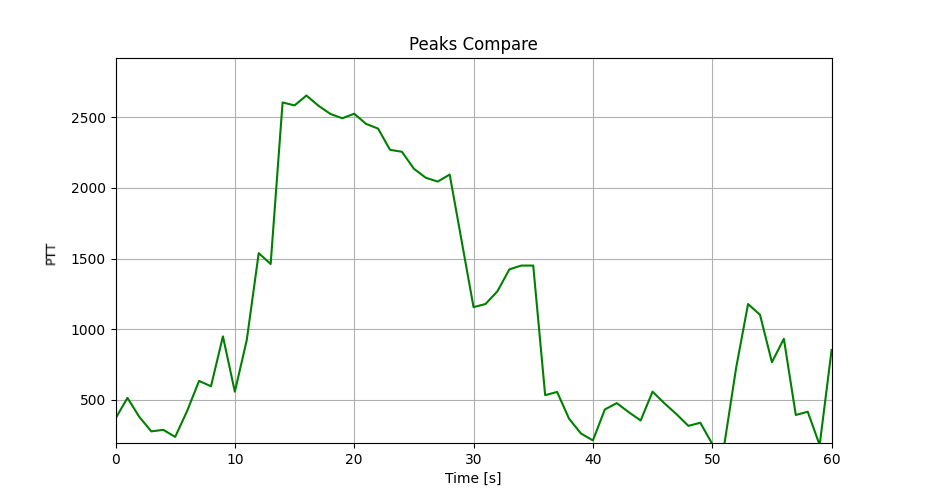
\includegraphics[width=1.0\linewidth]{images/Peaks_compare.png}
   \caption{Time differences between ECG and PPG peaks}%Chwilowe różnice czasowe między szczytami EKG i PPG
    \label{fig:PTT}
\end{figure}

Descriptive statistics were computed from the value vector, including the mean, which defines the average time of the heart rate phase shift, and the standard deviation, which represents its variability.

\subsection{HRV indicators}
Gaps between consecutive heartbeats were analyzed independently in both signals. Relative time was used in electrocardiography, resulting from windowed processing of the samples, whereas in the photoplethysmography system, timestamps were employed to ensure consistency with the recorded waveform and to allow synchronization with different data sources. RR intervals were determined from the ECG recordings, corresponding to the distances between R peaks. For PPG, IBI (Inter-Beat Interval) distances were computed. Based on these values, standard HRV parameters were calculated in RR form, and analogous calculations were performed for IBI.

\noindent\textit{1) Average RR interval length:} 
Arithmetic mean of RR intervals expressed with the Formula (4):
\begin{equation}
    Mean = \frac{1}{N} \sum_{i=1}^{N} RR_i
\end{equation}
where $RR_i$ -- $i$-th RR interval, and $N$ – analyzed interval count.

\noindent\textit{2) NN intervals standard deviation:} 
Total heart rate variability value, calculated based on all RR intervals expressed with the Formula (5):%Wielkość całkowitej zmienności rytmu serca, obliczana na podstawie wszystkich interwałów RR, wyrażona wzorem (5):
\begin{equation}
    SDNN = \sqrt{\frac{1}{N-1} \sum_{i=1}^{N} (RR_i - Mean)^2}
\end{equation}
where $Mean$ – average RR interval length, $RR_i$ – $i$-th RR interval, a $N$ – analyzed interval count. 
\newpage
\noindent\textit{3) Square root of averaged squares of differences between subsequent NN intervals:} 
Benchmark used in short-term heart rate fluctuations assessment expressed with the Formula (6):
\begin{equation}
    RMSSD = \sqrt{\frac{1}{N-1} \sum_{i=1}^{N-1} (RR_{i+1} - RR_i)^2}
\end{equation}
where $RR_i$ -- $i$-th RR interval, a $N$ – analyzed interval count.

% --- SECTION 4: Experimental Setup ---
\section{Experimental Setup and Data}

\subsection{ECG Data Acquisition}
Data used for R-peak detection model training and validation was acquired using the Polar H10 heart monitor, which is capable of recording electrocardiographic signals at a sampling frequency of 130 Hz. This resolution enables the creation of a profile essential for HRV analysis. The Polar H10 sensor is a heart rate detector commonly used in sports and diagnostics. The device employs chest electrodes to register electric potentials associated with cardiac activity, providing higher measurement precision compared to optical methods. Data transmission is carried out via the Bluetooth Low Energy (BLE) standard, while internal memory allows offline storage of recordings. The accuracy of the Polar H10 is comparable to that of single-channel ECG systems used in clinical diagnostics, making mobile signal acquisition feasible \cite{21}.

To collect the training dataset, eight measurement sessions were conducted with five participants. Each recording contained approximately 230,000 samples, corresponding to about 30 minutes of continuous signal per session. Data was transmitted in real time in 13-point packets, consistent with the established sampling rate, and subsequently stored in CSV format. These recordings captured varied heart rate dynamics and were used exclusively for model training to prevent data leakage.

\subsection{PPG Data Acquisition}
\paragraph{Mobile application}
An Android-based application utilizing the photoplethysmographic method for heart rate measurement was developed. Signal acquisition was performed by placing the participant’s fingertip directly on the camera lens, illuminated by the integrated LED light source. This setup enabled the detection of optical changes caused by cyclical variations in blood volume within the skin’s microvascular vessels. 

\begin{figure}[htbp]
    \centering
    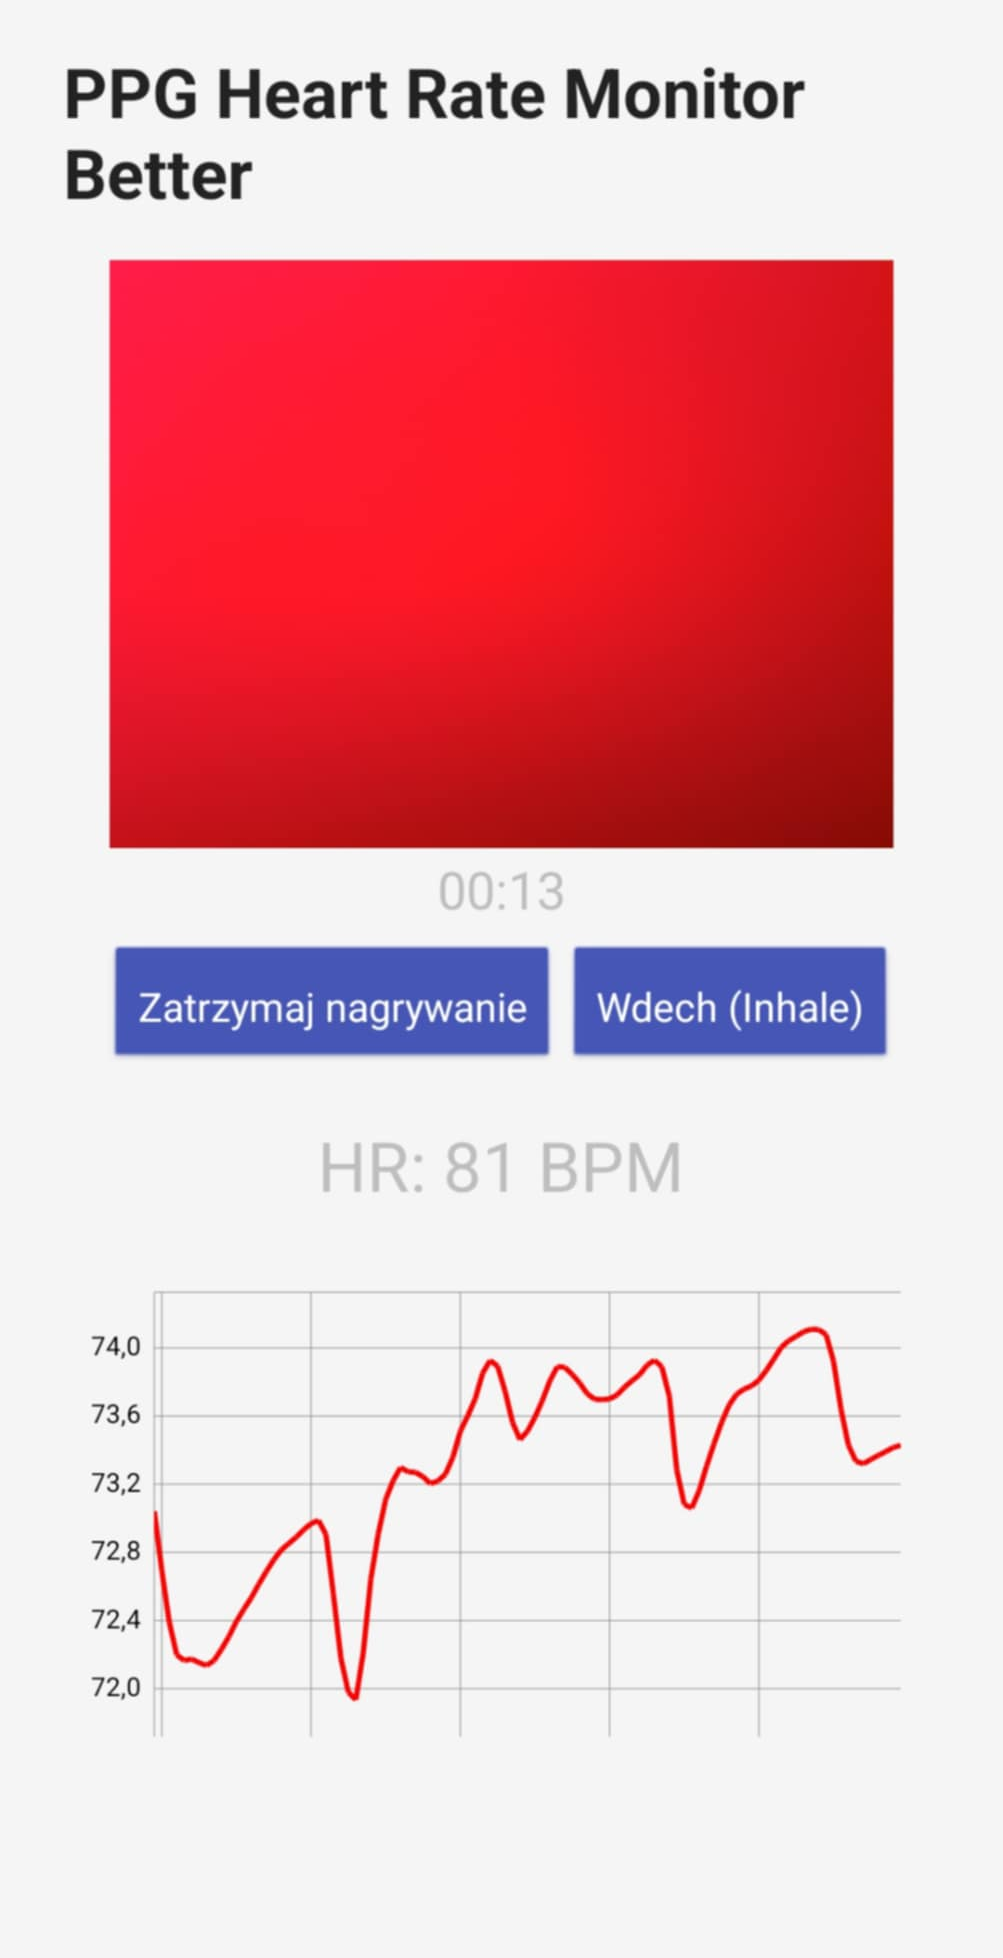
\includegraphics[scale=0.17]{images/aplikacja.png}
    \caption{Mobile app interface}
    \label{fig:aplikacja_mobilna}
\end{figure}

The application provides a user interface enabling real-time PPG waveforms visualization, as illustrated in Fig.~\ref{fig:aplikacja_mobilna}. The upper part of the screen contains a rectangular area displaying the video stream from the smartphone’s rear camera. A uniform red background indicates proper lens occlusion. Below the preview panel, a dynamic signal plot is presented and updated at the sampling frequency, allowing observation of cyclic amplitude variations corresponding to successive heartbeats. The interface includes a “Wdech/Inhale” button, designed as a manual respiratory marker. While this control allows users to tag inhalation onset times, the respiratory analysis was outside the scope of the peak detection performance evaluation presented in this study.

The recorded signal is processed using a low-pass filter. Peak detection is performed by analyzing three consecutive samples of the signal, where the central point is classified as a peak if its value exceeds that of its neighboring points. To prevent false identifications caused by motion artifacts, a newly detected peak is only acknowledged if it occurs at least 600 ms after the previous one. Each identified extremum is stored together with its timestamp and subsequently used to dynamically calculate the Beats Per Minute (BPM) according to Equation (1):

\begin{equation}
\text{BPM} = \frac{60}{\Delta t}
\label{eq:bpm}
\end{equation}
where $\Delta t$  - average time span between consecutive signal peaks

The source code of the developed mobile application has been hosted at the address: \\
\url{https://github.com/JanBancerewicz/PPGbetter}

\paragraph{Signal recording method}
Data used to train and validate the wave peak detection model was acquired using the developed application. Images were captured in real time in the YUV 4:2:0 format at a resolution of 640×480 pixels. From each frame, the luma component was extracted, and the average brightness value was computed. The resulting value represents a single sample of the raw photoplethysmographic signal.

Data acquisition was divided into training and validation phases to ensure result reliability. For model training, separate recording sessions were conducted using the mobile application, capturing 10-minute sessions of raw PPG signal, with small finger movements also taken into account. For validation, synchronized ECG and PPG signals were recorded simultaneously. This resulted in aligned datasets allowing for precise, sample-to-sample performance evaluation on data unseen during the training process.

Data transmission between the smartphone and the server was carried out using the WebSocket protocol. The data was sent in packets containing individual measurement points along with their corresponding timestamps. The sampling frequency was consistent with the frame rate, averaging about 30 Hz. The received data was buffered on the server and stored in CSV format.

% --- SECTION 5: Results ---
\section{Results and Discussion}

\subsection{R peak detection accuracy verification}
The performance of the convolutional network architecture for R peak detection in electrocardiographic signals was evaluated against the classic Pan-Tompkins algorithm and reference R peaks obtained using the NeuroKit library, which serves as a gold standard. The signal was sampled at 130 Hz and processed in nonoverlapping segments containing 256 samples.

The total number of detected maxima was 54 for the model, 56 using the Pan-Tompkins method, and 56 for the reference data. The results are presented in Table~\ref{tab:peak_comparison}, showing the number of True Positives, False Positives, and False Negatives, as well as the computed precision, sensitivity, and F1 scores, with a tolerance corresponding to 1–2 waveform samples. Visual comparisons of the detection performance are shown in Figure~\ref{fig:ai_pan-tompkins} and Figure~\ref{fig:ai_real_peaks}.

\begin{table}[ht]
\caption{Extrema detecting techniques assessment}
\label{tab:peak_comparison}
\centering
\begin{tabular}{|p{3.08cm}|c|c|c|c|c|c|}
\hline
\textbf{Method} & \textbf{TP} & \textbf{FP} & \textbf{FN} & \textbf{Prec.} & \textbf{Sens.} & \textbf{F1} \\
\hline
AI vs Pan-Tompkins & 54 & 0 & 2 & 1.000 & 0.964 & 0.982 \\
AI vs NeuroKit & 53 & 1 & 3 & 0.981 & 0.946 & 0.964 \\
Pan-Tompkins vs NeuroKit & 55 & 1 & 1 & 0.982 & 0.982 & 0.982 \\
\hline
\end{tabular}
\end{table}

\begin{figure}[htbp]
    \centering
    
\includegraphics[scale=0.2]{images/ai_pan-tompkins.png}
    \caption{Comparison of R peak detection between the network and Pan-Tompkins algorithm}
    \label{fig:ai_pan-tompkins}
\end{figure}

\begin{figure}[htbp]
    \centering
    
\includegraphics[scale=0.2]{images/ai_real_peaks.png}
    \caption{Comparison of R peak detection between the network and reference peaks}
    \label{fig:ai_real_peaks}
\end{figure}

The network’s performance in detecting R peaks is comparable to the classic Pan-Tompkins algorithm and shows high agreement with the reference values. Discrepancies resulting from missed or shifted peaks can be reduced through optimized signal preprocessing or further model training. Current machine learning systems are capable of achieving high performance in the automated detection of local peaks in electrocardiographic signals.

%Weryfikacja skuteczności detekcji pików fali
\subsection{Wave peak detection accuracy verification}
Peak identification in photoplethysmographic waveforms was performed using the convolutional network and a reference signal obtained through band-pass filtering and local maximum detection. The data were divided into segments of 100 samples each and normalized to the range [-1, 1]. In windowed mode, the model predictions were converted into point indices corresponding to potential wave peaks.

The machine learning algorithm detected 76 peaks, while the reference set contained 72. Detection performance was evaluated within a tolerance window of 264 ms, corresponding to 8 samples at a sampling rate of 30 Hz, using True Positive, False Positive, and False Negative metrics. The model produced 61 TP, 15 FP, and 11 FN, resulting in a precision of 0.803, a sensitivity of 0.847, and an F1 score of 0.824.

%Porównanie detekcji pików fali przez sieć splotową z szczytami referencyjnymi
\begin{figure}[htbp]
    \centering
    
\includegraphics[scale=0.28]{images/ppg_ai_vs_real.png}
    \caption{Peak detection comparison between the convolutional network and reference peaks}
    \label{fig:ppg_ai_real_peaks}
\end{figure}

%\newpage
The results, as illustrated in Figure~\ref{fig:ppg_ai_real_peaks}, indicate a high agreement between the network and the reference photoplethysmographic waveform maxima. The low number of false detections was primarily due to interferences and limitations of short-segment analysis. These results suggest the practical utility of the network in digital biomedical signal processing.

\subsection{HRV Analysis Results}

HRV parameters were calculated dynamically using a 60-second moving window. The results are presented in Figure~\ref{fig:hrv_ppg} for the PPG signal and Figure~\ref{fig:hrv_ecg} for the reference ECG signal. Each figure is divided into three panels illustrating the time course of key metrics:

\begin{itemize}
    \item \textbf{Panel (a)} shows the \textbf{Average RR interval length}. This metric reflects the instantaneous heart rate; rhythmic fluctuations visible in this plot typically correspond to respiratory sinus arrhythmia.
    \item \textbf{Panel (b)} presents the \textbf{SDNN} (Standard Deviation of NN intervals). This parameter measures total heart rate variability and indicates the overall autonomic nervous system activity over the analyzed window.
    \item \textbf{Panel (c)} displays the \textbf{RMSSD} (Root Mean Square of Successive Differences). This metric reflects short-term variations in heart rate and is primarily associated with parasympathetic activity.
\end{itemize}

\begin{figure}[htbp]
    \centering
    \begin{subfigure}{0.48\textwidth}
        \centering
        
\includegraphics[width=\linewidth]{images/Mean.png}
        \caption{Average RR interval length}
    \end{subfigure}
    
    \vspace{0.2cm} 
    \begin{subfigure}{0.48\textwidth}
        \centering
        
\includegraphics[width=\linewidth]{images/SDNN.png}
        \caption{Standard deviation of NN intervals (SDNN)}
    \end{subfigure}
    
    \vspace{0.2cm}  
    \begin{subfigure}{0.48\textwidth}
        \centering
        
\includegraphics[width=\linewidth]{images/RMSSD.png}
        \caption{Square root of average of squares of differences (RMSSD)}
    \end{subfigure}  
    \caption{Waveforms of HRV indicators computed for the \textbf{PPG signal}. }
    \label{fig:hrv_ppg}
\end{figure}

For comparison, the same set of HRV indicators computed from the reference ECG signals is presented below.

\begin{figure}[htbp]
    \centering
    \begin{subfigure}{0.48\textwidth}
        \centering
        
\includegraphics[width=\linewidth]{images/MEAN_EKG.png}
        \caption{Average RR interval length (ECG)}
    \end{subfigure}
    
    \vspace{0.2cm} 
    \begin{subfigure}{0.48\textwidth}
        \centering
        
\includegraphics[width=\linewidth]{images/SDNN_EKG.png}
        \caption{Standard deviation of NN intervals (SDNN) (ECG)}
    \end{subfigure}
    
    \vspace{0.2cm}  
    \begin{subfigure}{0.48\textwidth}
        \centering
        % POPRAWKA: Dodano folder images/ przed nazwą pliku
        
\includegraphics[width=\linewidth]{images/RMSSD_EKG.png}
        \caption{Square root of average of squares of differences (RMSSD) (ECG)}
    \end{subfigure}  
    \caption{Waveforms of HRV indicators calculated for the \textbf{reference ECG}.}
    \label{fig:hrv_ecg}
\end{figure}

Comparison of HRV indicators between PPG and ECG methods (see Figure~\ref{fig:hrv_ppg} and Figure~\ref{fig:hrv_ecg}) showed that RMSSD and SDNN values calculated from ECG were more stable and less prone to sudden fluctuations. In the case of PPG, greater variability and occasional outlier values were observed. A possible explanation is the method’s susceptibility to interferences, such as variations in finger pressure against the camera.
Despite the greater variability in PPG waveforms, the average HRV indicator values (SDNN and RMSSD) are similar to those obtained from ECG. This finding confirms that, under proper recording conditions, PPG can serve as a reliable alternative to ECG for heart rate variability analysis, although it requires additional filtering and artifact compensation.

\section{Summary}
Evaluation has shown that convolutional and recurrent architectures provide a high level of agreement with classical methods and reference data while minimizing false detections. The proposed models achieved high precision in detecting key points in the signals, with the F1 score reaching 0.9753 for R peaks in ECG signals and 0.9774 for wave peaks in PPG waveforms. The high accuracy of peak detection in photoplethysmographic signals demonstrates the strong potential of this method for reliably estimating IBIs, which are the counterparts of RR intervals in ECG signals.


Biomedical signal recording systems powered by machine learning methods show high potential for real-time health monitoring. Future efforts should focus on increasing the robustness of algorithms against environmental interferences, including motion artifacts, noise, and varying physiological conditions. It is also essential to develop mechanisms that enable integration with advanced telemedicine systems for continuous data uploading and analysis. Implementing these solutions could facilitate early identification of cardiac disorders and support clinical decision-making.

A specific design choice in the developed mobile application was the imposition of a 600 ms refractory period between detected peaks. While this constraint limits the maximum detectable heart rate to approximately 100 BPM, it was implemented as a deliberate denoising strategy for resting-state measurements. In non-clinical mobile PPG acquisition, camera sensor noise and micro-movements often manifest as high-frequency artifacts that can mimic rapid heartbeats. By enforcing this threshold, the system significantly reduces false positive detections, prioritizing the high precision required for HRV metrics (such as SDNN and RMSSD) over the ability to monitor intensive physical exertion.
% #2 dodatek tłumaczący wybór próbkowania 600ms w appce 

It is worth noting, however, that although the models have been trained on data that included interferences like sudden bodily movements or small finger shifting, their validation happened in a controlled environment. This highlights an important limitation — uncertainty remains regarding the system’s performance in real-world conditions, especially during intensive physical activity where movement becomes a dominating source of interferences. This problem is particularly clear in the PPG signal where unstable contact of the detector with the skin and ambient light interference may lead to significant measurement errors. There may exist improvements which would reduce the impact of the interferences on the results such as: applying adaptation filters which would dynamically correct their effect to account for the noise characteristic in the signal or usage of more complex deep learning models to process a variety of data.
% #2 miniaturowe dodanie "ambient light interference"

%\newpage

The developed system, including the source code, has been made publicly available on GitHub at the following repositories:

\noindent
\href{https://github.com/JanBancerewicz/PPGbetter}{https://github.com/JanBancerewicz/PPGbetter} \\
\href{https://github.com/JanBancerewicz/research-project}{https://github.com/JanBancerewicz/research-project}.

%\newpage

\begin{thebibliography}{1}

\bibitem{1}
J. D. Bronzino and D. R. Peterson, Eds., \emph{The Biomedical Engineering Handbook}, 4th ed., vol. 3: Biomedical Signals, Imaging, and Informatics, CRC Press, Boca Raton, 2015.

\bibitem{2}
R. R. Sharma and R. B. Pachori, "Baseline wander and power line interference removal from ECG signals using eigenvalue decomposition," \emph{Biomedical Signal Processing and Control}, vol. 45, 2018, doi: 10.1016/j.bspc.2018.05.002.

\bibitem{3}
L. Sörnmo and P. Laguna, \emph{Bioelectrical Signal Processing in Cardiac and Neurological Applications}, Academic Press (Elsevier), Amsterdam, 2005.

\bibitem{4}
P. Podder, M. M. Hasan, M. R. Islam, and M. Sayeed, "Design and implementation of Butterworth, Chebyshev-I and elliptic filter for speech signal analysis," \emph{International Journal of Computer Applications}, vol. 975, no. 8887, 2020, doi: 10.48550/arXiv.2002.03130.

\bibitem{5}
M. R. Keshtkaran and Z. Yang, "A fast, robust algorithm for power line interference cancellation in neural recording," \emph{Journal of Neural Engineering}, vol. 11, no. 2, Art. no. 026017, 2014, doi: 10.1088/1741-2560/11/2/026017.

\bibitem{6}
S. K. Mitra, \emph{Digital Signal Processing: A Computer-Based Approach}, 4th ed., McGraw-Hill Education, New York, 2011.

\bibitem{7}
Y. Yue, C. Chen, X. Wu, and X. Zhou, "An effective electrocardiogram segments denoising method combined with ensemble empirical mode decomposition, empirical mode decomposition, and wavelet packet," \emph{IET Signal Processing}, vol. 17, no. 6, 2023, doi: 10.1049/sil2.12232.

\bibitem{8}
S. Haykin, \emph{Adaptive Filter Theory}, 5th ed., Pearson, London, 2013.

\bibitem{9}
A. Hyvärinen and E. Oja, "Independent component analysis: algorithms and applications," \emph{Neural Networks}, vol. 13, no. 4–5, 2000, doi: 10.1016/S0893-6080(00)00026-5.

\bibitem{10}
O. Faust, Y. Hagiwara, T. J. Hong, O. S. Lih, and U. R. Acharya, "Deep learning for healthcare applications based on physiological signals: A review," \emph{Computer Methods and Programs in Biomedicine}, vol. 161, 2018, doi: 10.1016/j.cmpb.2018.04.005.

\bibitem{11}
A. Boulif, B. Ananou, M. Ouladsine, and S. Delliaux, "A literature review: ECG-based models for arrhythmia diagnosis using artificial intelligence techniques," \emph{Bioinformatics and Biology Insights}, vol. 17, Art. no. 11779322221149600, 2023, doi: 10.1177/11779322221149600.

\bibitem{12}
Z. Ebrahimi, M. Loni, M. Daneshtalab, and A. Gharehbaghi, "A review on deep learning methods for ECG arrhythmia classification," \emph{Expert Systems with Applications: X}, vol. 7, Art. no. 100033, 2020, doi: 10.1016/j.eswax.2020.100033.

\bibitem{13}
D. A. Coast, R. M. Stern, G. G. Cano, and S. A. Briller, "An approach to cardiac arrhythmia analysis using hidden Markov models," \emph{IEEE Transactions on Biomedical Engineering}, vol. 37, no. 9, 1990, doi: 10.1109/10.58593.

\bibitem{14}
K. Kazemi, J. Laitali, I. Azimi, P. Liljeberg, and A. M. Rahmani, "Robust PPG Peak Detection Using Dilated Convolutional Neural Networks," \emph{Sensors}, vol. 22, no. 16, Art. no. 6054, 2022, doi: 10.3390/s22166054.

\bibitem{15}
S. Ikram, A. Ikram, H. Singh, M. D. A. Awan, S. Naveed, I. De la Torre Díez, H. F. Gongora, and T. C. Chio Montero, "Transformer-based ECG classification for early detection of cardiac arrhythmias," \emph{Frontiers in Medicine}, vol. 12, Art. no. 1600855, 2025, doi: 10.3389/fmed.2025.1600855.

\bibitem{16}
C. V. Nguyen and C. D. Do, "Transfer learning in ECG diagnosis: Is it effective?" \emph{PLOS ONE}, vol. 20, no. 5, Art. no. e0316043, 2025, doi: 10.1371/journal.pone.0316043.

\bibitem{17}
W. Wang and L. Najafizadeh, "Ultra-short term heart rate variability estimation using PPG and end-to-end deep learning," in \emph{Proceedings of the 58th Asilomar Conference on Signals, Systems and Computers (ACSSC)}, 2024, doi: 10.1109/IEEECONF60004.2024.10943067.

\bibitem{18}
J. Xu, Y. Zhang, W. Wang, M. Xie, and D. Zhu, "A Comprehensive PPG-based Dataset for HR/HRV Studies," in \emph{Proceedings of the 13th IEEE International Conference on Healthcare Informatics}, 2025, doi: 10.48550/arXiv.2505.18165.

\bibitem{19}
B. De Ridder, B. Van Rompaey, J. K. Kampen, S. Haine, and T. Dilles, "Smartphone apps using photoplethysmography for heart rate monitoring: meta-analysis," \emph{JMIR Cardio}, vol. 2, no. 1, 2018, doi: 10.2196/cardio.8802.

\bibitem{20}
J. D. Mather, L. D. Hayes, J. L. Mair, and N. F. Sculthorpe, "Validity of resting heart rate derived from contact-based smartphone photoplethysmography compared with electrocardiography: a scoping review and checklist for optimal acquisition and reporting," \emph{Frontiers in Digital Health}, vol. 6, Art. no. 1326511, 2024, doi: 10.3389/fdgth.2024.1326511.

\bibitem{21} 
M. Schaffarczyk, B. Rogers, R. Reer, and T. Gronwald, "Validity of the Polar H10 sensor for heart rate variability analysis during resting state and incremental exercise in recreational men and women," \emph{Sensors}, vol. 22, no. 17, Art. no. 6536, 2022, doi: 10.3390/s22176536.

\bibitem{22} 
W. M. Laghari, M. U. Baloch, M. A. Mengal, and S. J. Shah, "Performance analysis of analog Butterworth low pass filter as compared to Chebyshev Type-I filter, Chebyshev Type-II filter and elliptical filter," \emph{Circuits and Systems}, vol. 5, no. 9, 2014, doi: 10.4236/cs.2014.59023.
%W. M. Laghari, M. Baloch, M. Mengal, S. Shah, “Performance Analysis of Analog Butterworth Low Pass Filter as Compared to Chebyshev Type-I Filter, Chebyshev Type-II Filter and Elliptical Filter”

\bibitem{23} 
S. Chakraborty, K. K. Jha, and A. Patra, "Design of IIR digital highpass Butterworth filter using analog to digital mapping technique," \emph{International Journal of Computer Applications}, vol. 52, no. 7, 2012, doi: 10.5120/8212-1630.
%S. Chakraborty, K. K. Jha, A. Patra, “Design of IIR Digital Highpass Butterworth Filter using Analog to Digital Mapping Technique”

\bibitem{24} 
G. Lenis, N. Pilia, A. Loewe, W. H. W. Schulze, and O. Dössel, "Comparison of baseline wander removal techniques considering the preservation of ST changes in the ischemic ECG: A simulation study," \emph{Computational and Mathematical Methods in Medicine}, Art. no. 9295029, 2017, doi: 10.1155/2017/9295029.
%G. Lenis, N. Pilia, A. Loewe, W. H. W. Schulze, O. Dössel, “Comparison of Baseline Wander Removal Techniques considering the Preservation of ST Changes in the Ischemic ECG: A Simulation Study”

\bibitem{25} 
R. J. Martis, U. R. Acharya, and H. Adeli, "Current methods in electrocardiogram characterization," \emph{Computers in Biology and Medicine}, vol. 48, 2014, doi: 10.1016/j.compbiomed.2014.02.012.
%R. J. Martis, U. R. Acharya, H. Adeli, “Current methods in electrocardiogram characterization”

\bibitem{26} 
M. A. F. Pimentel, A. E. W. Johnson, P. H. Charlton, D. Birrenkott, P. J. Watkinson, L. Tarassenko, and D. A. Clifton, "Toward a robust estimation of respiratory rate from pulse oximeters," \emph{IEEE Transactions on Biomedical Engineering}, vol. 64, no. 8, 2016, doi: 10.1109/TBME.2016.2613124.
%M. A. F. Pimentel et al., “Toward a robust estimation of heart rate from wrist-type PPG signals”, 2016

\bibitem{27} 
J. Pan and W. J. Tompkins, "A real-time QRS detection algorithm," \emph{IEEE Transactions on Biomedical Engineering}, vol. 32, no. 3, 1985, doi: 10.1109/TBME.1985.325532.
%J. Pan and W. J. Tompkins, “A real-time QRS detection algorithm”
\end{thebibliography}
\end{document}
